\section{Design}

In questa sezione si trovano dei diagrammi volti a modellizare la navigazione all'interno dell'applicazione.

\subsection{UX Diagrams}

Gli UX Diagrams mostrano una visione delle schermate, degli eventi e delle funzionalità che caratterizzano l'esperienza dell'utente durante l'uso del sistema. Avremo quindi "screen" per modellizzare le schermate e gli "input form" che mostrano dei moduli soggetti a compilazione, essi vanno a rappresentare gli stereotipi del modello UX, tramite le frecce possono essere invece indicati degli eventi oppure l'attivazione di un metodo, l'essere orientate o meno va a sottointendere la direzione di navigazione. 
Ogni entità può essere dotata di attributi e metodi qualora vadano a modificare lo stato del sistema. 

Tratteremo questo tipo di modellizzazione dai 3 differenti punti di vista possibili nell'uso di SWIM ossia quelli dell' ospite, dell'utente registrato e dell'amministratore.

\subsubsection{UX per un ospite}

Analizzeremo innanzitutto la navigazione dell'ospite, che ricordiamo può compiere ricerche all'interno dell'applicazione, visionare il contenuto dei thread, registrarsi ed eventualmente procedere con l'accesso al sistema da utente registrato. 

\begin{figure} [!hbtp]
\centering
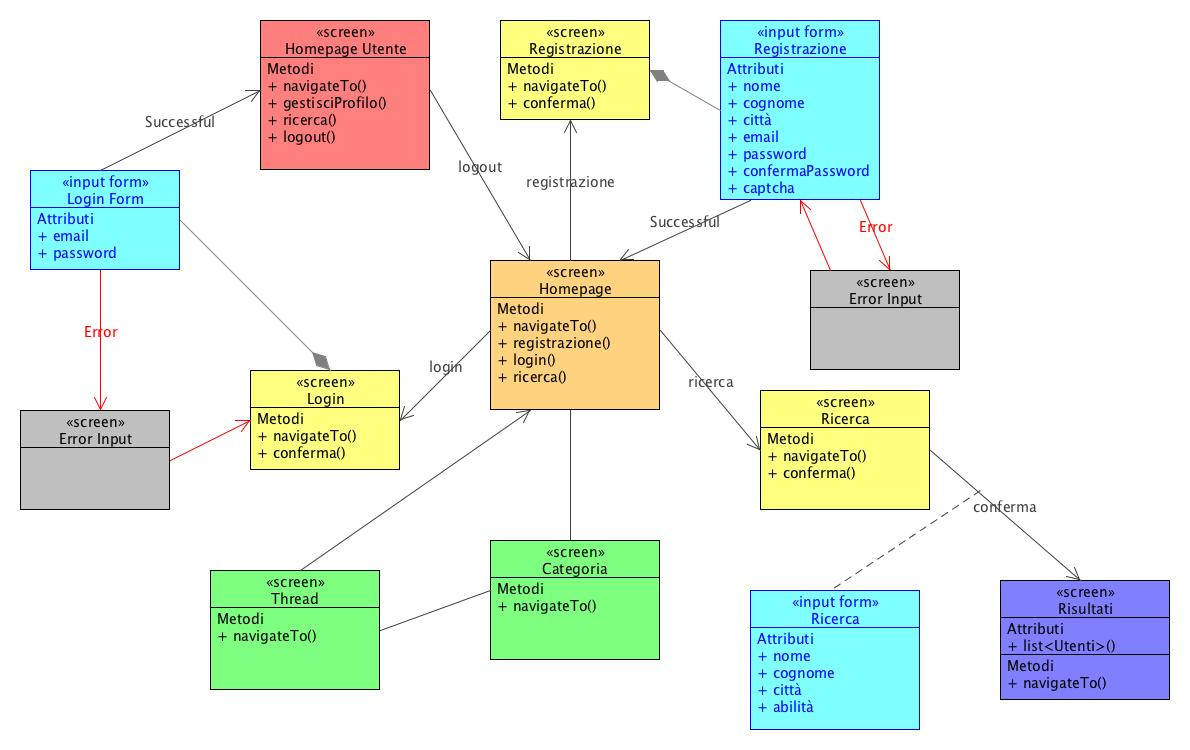
\includegraphics[scale=0.40]{uxEsperienzaOspite.jpg} \\
\caption{\label{uxOspite} Modello di navigazione all'interno di SWIM da parte di un ospite }
\end{figure}

\begin{itemize}
\item[$\textcolor{red}{\diamondsuit}$] I moduli della registrazione e dell'accesso sono stati modellati come classi contenute per descrivere l'eventuale meccanismo di reindirizzamento nel caso sia presente una casistica di errore. 
\item[$\textcolor{red}{\diamondsuit}$] Il modulo di ricerca invece è stato risolto come classe associata ad associazione in quanto la ricerca nell' eventualità sfortunata porta ad una lista risultante nulla.
\item[$\textcolor{red}{\diamondsuit}$] L' Homepage è stata identificata come riferimento principale in quanto è il fulcro della maggior parte delle diverse sequenze che si possono realizzare, come si può notare il colore è distinto rispetto a quello dell' Homepage Utente che in questa modellizzazione iniziale rappresenta solo una destinazione dalla quale non avverrà altro se non l'operazione di logout.
\item[$\textcolor{red}{\diamondsuit}$] In giallo sono state colorate le schermate che rappresentano le effettive operazioni che può svolgere l'ospite, mediante le quali interagirà con il database. 
\item[$\textcolor{red}{\diamondsuit}$] In verde invece le schermate attraverso le quali l'ospite potrà navigare con il solo scopo di leggere.
\end{itemize}

\pagebreak

\subsubsection{UX per un utente registrato}

Passiamo adesso ad un' analisi riguardante la navigazione con i privilegi degli utenti registrati, dopo aver effettuato l'autentificazione infatti, potranno svolgere attività quali la gestione del loro profilo, l'invio di messaggi privati, la partecipazione attiva ai thread tramite messaggi pubblici e l'inviare e richiedere amicizie agli altri utenti di SWIM.  

\begin{figure} [!hbtp]
\centering
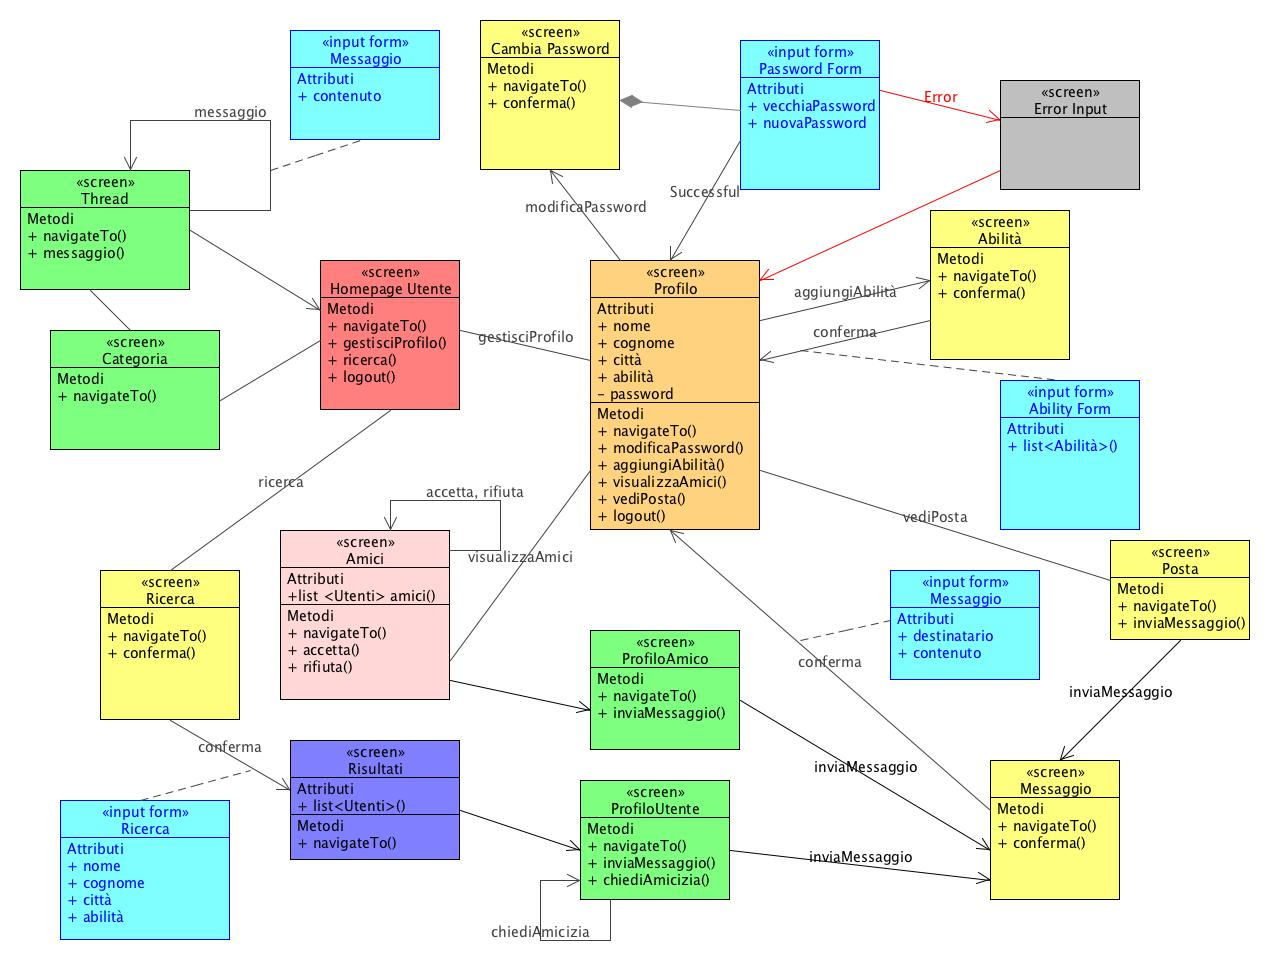
\includegraphics[scale=0.40]{uxEsperienzaRegistrato.jpg} \\
\caption{\label{uxRegistrato} Modello di navigazione all'interno di SWIM da parte di un utente registrato }
\end{figure}

\begin{itemize}
\item[$\textcolor{red}{\diamondsuit}$] Per questo modello il fulcro è il Profilo in quanto da esso è possibile compiere la maggior parte delle attività privilegiate dell'utente autenticato.
\item[$\textcolor{red}{\diamondsuit}$] Il modulo per la modifica della password è stato rappresentato con una classe contenuta per sottolineare la possibilità di immettere una password vecchia errata.
\item[$\textcolor{red}{\diamondsuit}$] Il modulo per la modifica delle abilità è stato modellato con una classe associata ad associazione in quanto l'aggiunta di abilità alle propie facoltà avrà sempre esito positivo.
\item[$\textcolor{red}{\diamondsuit}$] Anche i moduli per la scrittura dei messaggi privati e pubblici sono stati modellati con classi associate ad associazione, i messaggi non incorrono in casistiche di errore grazie al fatto che, ove necessario, il campo destinatario sarà completato tramite selezione dalla lista amici o autoimmissione da parte del sistema. 
\item[$\textcolor{red}{\diamondsuit}$] Gli autoanelli indicano azioni che possono essere compiute e che vanno quindi a modificare lo stato del sistema, la particolarità è data dal fatto che sarà visualizzata la stessa schermata, nella quale saranno presenti le eventuali modifiche.
\item[$\textcolor{red}{\diamondsuit}$] Le convenzioni usate per i colori sono le medesime del diagramma precedente.
\end{itemize}


\subsubsection{UX per un amministratore}

Infine trattiamo la navigazione da parte di un amministratore, per semplicità di lettura, sarà modellata solo l'attività più importante che lo contraddistingue da un utente registrato ossia la facoltà di creare nuove abilità che saranno quindi disponibili all'utenza di SWIM.

\begin{figure} [!hbtp]
\centering
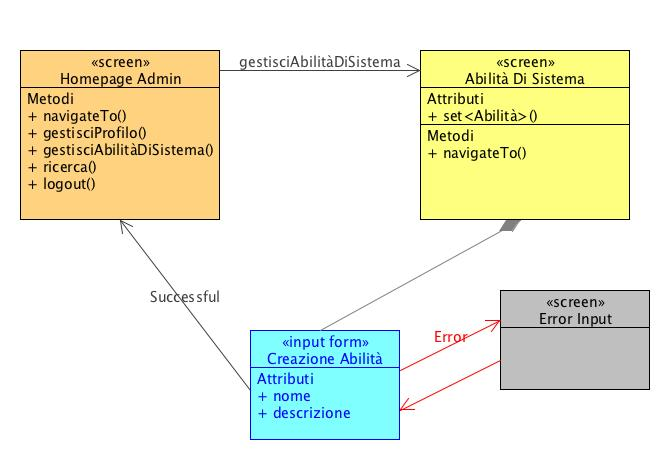
\includegraphics[scale=0.40]{uxEsperienzaAmministratore.jpg} \\
\caption{\label{uxAmministratore} Modello di navigazione da parte di un amministratore di SWIM}
\end{figure}

\begin{itemize}
\item[$\textcolor{red}{\diamondsuit}$] Il modulo per la creazione di una nuova abilità è stato realizzato mediante una classe contenuta per tener conto dell'eventualità che possa essere immesso il nome di un' abilità già esistente.
\end{itemize}
